\documentclass[11pt,a4paper]{article}
\usepackage[margin=1.9cm]{geometry}
\usepackage[T1]{fontenc}
\usepackage{lmodern}
\usepackage{microtype}
\usepackage{setspace}
\setstretch{1.08}
\usepackage{amsmath,amssymb}
\usepackage{booktabs}
\usepackage{tabularx}
\usepackage{xcolor}
\usepackage{tikz}
\usetikzlibrary{arrows.meta,positioning,fit,backgrounds,calc,shapes.geometric}
\usepackage{pgfplots}
\pgfplotsset{compat=1.18}
\usepackage[hyphens]{url}
\usepackage{hyperref}
\usepackage{enumitem}
\usepackage{listings}
\usepackage{fancyhdr}
\usepackage{titlesec}
\usepackage{tcolorbox}
\tcbuselibrary{skins,breakable}

% Spacing & typography adjustments
\titlespacing*{\section}{0pt}{14pt plus 2pt minus 2pt}{6pt plus 1pt minus 1pt}
\titlespacing*{\subsection}{0pt}{10pt plus 2pt minus 1pt}{4pt plus 1pt minus 1pt}
\titlespacing*{\subsubsection}{0pt}{7pt plus 1pt minus 1pt}{3pt}

\titleformat{\section}{\sffamily\Large\bfseries\color{darkblue}}{\thesection}{0.8em}{}
\titleformat{\subsection}{\sffamily\large\bfseries\color{sharededge}}{\thesubsection}{0.7em}{}
\titleformat{\subsubsection}{\sffamily\normalsize\bfseries\color{darkblue}}{\thesubsubsection}{0.6em}{}

\setlist{nosep,leftmargin=1.4em,itemsep=3pt}

% Custom Colors (Modern Flat Palette)
\definecolor{shared}{HTML}{EFF6FF}
\definecolor{sharededge}{HTML}{2563EB}
\definecolor{head}{HTML}{FEF3C7}
\definecolor{headedge}{HTML}{D97706}
\definecolor{io}{HTML}{F8FAFC}
\definecolor{ioedge}{HTML}{475569}
\definecolor{repbox}{HTML}{F5F3FF}
\definecolor{crep}{HTML}{7C3AED}
\definecolor{codebg}{HTML}{F8FAFC}
\definecolor{darkblue}{HTML}{0F172A}
\definecolor{boxborder}{HTML}{CBD5E1}
\definecolor{boxheader}{HTML}{1E293B}
\definecolor{emerald}{HTML}{059669}
\definecolor{emeraldbox}{HTML}{ECFDF5}

\hypersetup{
  colorlinks=true,
  linkcolor=sharededge,
  citecolor=sharededge,
  urlcolor=sharededge,
  pdfauthor={Amal Verma, Prathamesh Sankhe, Rupak R. Gupta, Vaishvi Khandelwal},
  pdftitle={Decide: Architecture & Engineering Manual}
}

% Callout Boxes (OSS Documentation Style)
\newtcolorbox{ossbox}[2][]{
  enhanced,
  breakable,
  colback=shared,
  colframe=sharededge,
  coltitle=white,
  fonttitle=\sffamily\bfseries\small,
  title={#2},
  arc=3pt,
  boxrule=1pt,
  left=7pt, right=7pt, top=6pt, bottom=6pt,
  #1
}

\newtcolorbox{tipbox}[2][]{
  enhanced,
  breakable,
  colback=emeraldbox,
  colframe=emerald,
  coltitle=white,
  fonttitle=\sffamily\bfseries\small,
  title={#2},
  arc=3pt,
  boxrule=1pt,
  left=7pt, right=7pt, top=6pt, bottom=6pt,
  #1
}

\newtcolorbox{warnbox}[2][]{
  enhanced,
  breakable,
  colback=repbox,
  colframe=crep,
  coltitle=white,
  fonttitle=\sffamily\bfseries\small,
  title={#2},
  arc=3pt,
  boxrule=1pt,
  left=7pt, right=7pt, top=6pt, bottom=6pt,
  #1
}

% Listings configuration
\lstset{
  backgroundcolor=\color{codebg},
  basicstyle=\fontsize{8.5pt}{11pt}\ttfamily,
  breaklines=true,
  breakatwhitespace=true,
  frame=single,
  rulecolor=\color{boxborder},
  keywordstyle=\color{sharededge}\bfseries,
  commentstyle=\color{gray!70}\itshape,
  stringstyle=\color{emerald},
  showstringspaces=false,
  tabsize=2
}

% TikZ Styles
\tikzset{
  layer/.style={draw=ioedge,fill=io,rounded corners=4pt,align=center,font=\small,inner sep=6pt,minimum width=3.8cm,minimum height=1.35cm},
  core/.style={draw=sharededge,fill=shared,rounded corners=4pt,align=center,font=\small\bfseries,inner sep=6pt,minimum width=4.0cm,minimum height=1.35cm},
  policy/.style={draw=headedge,fill=head,rounded corners=4pt,align=center,font=\small,inner sep=6pt,minimum width=4.0cm,minimum height=1.35cm},
  gov/.style={draw=crep,fill=repbox,rounded corners=4pt,align=center,font=\small,inner sep=6pt,minimum width=4.0cm,minimum height=1.35cm},
  arr/.style={-{Stealth[length=2.5mm]},thick,draw=darkblue},
  looparr/.style={-{Stealth[length=2.5mm]},thick,draw=crep},
}

\pagestyle{fancy}
\fancyhf{}
\renewcommand{\headrulewidth}{0.4pt}
\fancyhead[L]{\small\sffamily\textbf{Decide}: Architecture \& Engineering Reference Manual}
\fancyhead[R]{\small\sffamily Core Codebase Documentation}
\fancyfoot[C]{\thepage}

\title{\vspace{-1.2cm}\textbf{\huge Decide: Architecture \& Engineering Manual}\\[6pt]
\Large An In-Depth Technical Guide to the Sub-25\,ms CPU Decision Engine,\\Fused Multi-Task MoE Graph, and Decide v2 Adaptive Reputation System}

\author{
  \textbf{Amal Verma} (231080076) \quad
  \textbf{Prathamesh Sankhe} (231080061) \\[4pt]
  \textbf{Rupak R. Gupta} (231080028) \quad
  \textbf{Vaishvi Khandelwal} (231081074)
}
\date{November 2026}

\begin{document}
\maketitle

\begin{abstract}
\noindent
This document serves as the comprehensive engineering manual and source code reference for \textbf{Decide} (\path{Jev-router-decide}), an open-source, sub-25\,ms CPU-only decision service designed for automated customer support triage behind an HTTP REST API (\texttt{POST /v1/decide}). Rather than duplicating the high-level empirical results of the four-page research paper (\path{docs/report/report.tex}), this manual examines the operational implementation of every script, class, and pipeline module across the entire repository. The system executes three typed queries---\emph{route} (5-way queue triage), \emph{approve} (risk-asymmetric auto-approval with $3:1$ false-positive loss), and \emph{grounded} (knowledge-base factual verification)---in a single forward pass over a 92\,MB fused ONNX graph (MiniLM int8 + Ettin-17m fp32) on commodity multicore CPUs. We provide an exhaustive file-by-file analysis across seven core engineering subsystems: (1) Core Deep Learning Runtime \& Input Preprocessing, (2) Decide v2 Adaptive Reputation \& Integrity Gating, (3) Application Layer \& Zero-Dependency Web UI, (4) Multi-Task Training, Mixture-of-Experts Architecture \& Graph Surgery, (5) Calibration, Bayes Policy Optimization \& Analytical Tooling, (6) Validation, Dataset Auditing \& Benchmarking Harnesses, and (7) Automation, Shell Scripting \& CLI Utilities.
\end{abstract}

\vspace{0.1cm}
\tableofcontents
\vspace{0.4cm}
\hrule
\vspace{0.4cm}

\section{System Architecture and Repository Overview}

The Decide platform is designed to eliminate serving-time GPU requirements and runtime network dependencies. Inference executes on commodity multicore CPUs within a strict 25\,ms p95 latency envelope.

\subsection{Architectural Blueprint and Request Lifecycle}
Figure~\ref{fig:system_overview} illustrates the decoupled multi-tier architecture. Incoming JSON payloads are intercepted by the FastAPI gateway, validated via Pydantic, framed into contextual text pairs and 75-dimensional tabular feature vectors, evaluated in a single forward pass by a fused dual-model ONNX graph, filtered through a Bayes risk decision boundary, and fed back into an in-memory reputation ledger.

\begin{figure}[htbp]
\centering
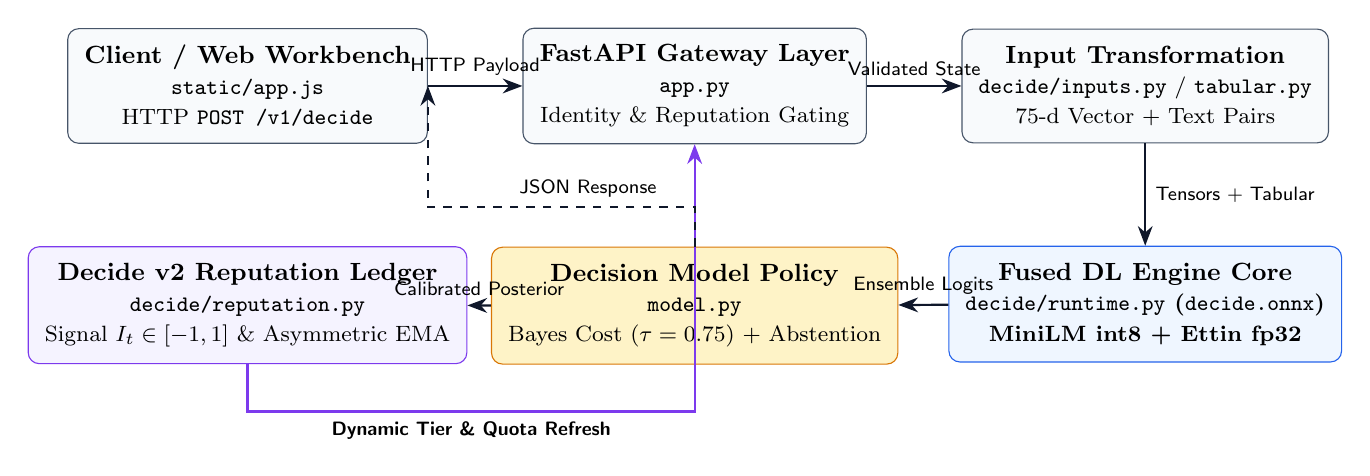
\begin{tikzpicture}[node distance=9mm and 12mm]
  % Top Row: Ingestion and Input Processing
  \node[layer] (client) {\textbf{Client / Web Workbench}\\\footnotesize\texttt{static/app.js}\\\footnotesize HTTP \texttt{POST /v1/decide}};
  \node[layer, right=of client] (gw) {\textbf{FastAPI Gateway Layer}\\\footnotesize\texttt{app.py}\\\footnotesize Identity \& Reputation Gating};
  \node[layer, right=of gw] (trans) {\textbf{Input Transformation}\\\footnotesize\texttt{decide/inputs.py} / \texttt{tabular.py}\\\footnotesize 75-d Vector + Text Pairs};

  % Middle Row: Deep Learning Core and Policy
  \node[core, below=of trans, yshift=-4mm] (engine) {\textbf{Fused DL Engine Core}\\\footnotesize\texttt{decide/runtime.py} (\texttt{decide.onnx})\\\footnotesize MiniLM int8 + Ettin fp32};
  \node[policy, below=of gw, yshift=-4mm] (model) {\textbf{Decision Model Policy}\\\footnotesize\texttt{model.py}\\\footnotesize Bayes Cost ($\tau=0.75$) + Abstention};

  % Bottom Row: Closed-Loop Governance
  \node[gov, below=of client, yshift=-4mm] (rep) {\textbf{Decide v2 Reputation Ledger}\\\footnotesize\texttt{decide/reputation.py}\\\footnotesize Signal $I_t \in [-1, 1]$ \& Asymmetric EMA};

  % Horizontal and Vertical Forward Flows
  \draw[arr] (client) -- node[above,font=\scriptsize\sffamily] {HTTP Payload} (gw);
  \draw[arr] (gw) -- node[above,font=\scriptsize\sffamily] {Validated State} (trans);
  \draw[arr] (trans) -- node[right,font=\scriptsize\sffamily] {Tensors + Tabular} (engine);
  \draw[arr] (engine) -- node[above,font=\scriptsize\sffamily] {Ensemble Logits} (model);
  \draw[arr] (model) -- node[above,font=\scriptsize\sffamily] {Calibrated Posterior} (rep);

  % Clean Collision-Free Feedback Loop (Routes along top/bottom margins, zero intersections)
  \draw[looparr] (rep.south) -- ++(0,-0.6) -| node[pos=0.25,below,font=\scriptsize\sffamily\bfseries] {Dynamic Tier \& Quota Refresh} (gw.south);

  % Response Output Flow
  \draw[arr, dashed] (model.north) -- ++(0,0.5) -| node[pos=0.2,above,font=\scriptsize\sffamily] {JSON Response} (client.east);
\end{tikzpicture}
\caption{Decide end-to-end multi-tier system architecture. The feedback loop dynamically adjusts client rate quotas and tarpit delays based on model verification veracity without intersecting inference layers.}
\label{fig:system_overview}
\end{figure}

\subsection{Subsystem Breakdown and Module Map}
The codebase is structured into seven distinct subsystems, detailed in Table~\ref{tab:subsystems_clean}.

\begin{table}[htbp]
\centering
\footnotesize
\renewcommand{\arraystretch}{1.15}
\begin{tabularx}{\linewidth}{>{\raggedright\arraybackslash}p{4.6cm} >{\raggedright\arraybackslash}X}
\toprule
\textbf{Subsystem Name \& Modules} & \textbf{Architectural Scope \& Primary Responsibilities} \\
\midrule
\textbf{1. DL Runtime \& Inputs}\\[1pt]
\texttt{decide/runtime.py}\\\texttt{model.py}\\\texttt{decide/inputs.py}\\\texttt{decide/tabular.py}\\\texttt{decide/features.py}\\\texttt{decide/baseline\_runtime.py} &
Executes CPU inference on the fused ONNX model graph via single-session \texttt{session.run()}, formats contextual cross-encoder sequence pairs, generates the 75-dimensional tabular cutoff vector, and enforces defensive empty-input guardrails.\\
\midrule
\textbf{2. Reputation Engine (v2)}\\[1pt]
\texttt{decide/reputation.py} &
Provides closed-loop client integrity governance, derives instant veracity signals $I_t \in [-1.0, 1.0]$, executes asymmetric EMA score updates, and manages rate quotas and tarpit queues.\\
\midrule
\textbf{3. API Layer \& Workbench}\\[1pt]
\texttt{app.py}\\\texttt{serve.py}\\\texttt{static/app.js}\\\texttt{static/index.html} &
Exposes production REST endpoints (\texttt{/v1/decide}, \texttt{/health}, \texttt{/v1/metrics}, \texttt{/v1/reputation}) with Pydantic validation, launches Uvicorn workers, and serves an offline interactive UI workbench.\\
\midrule
\textbf{4. Multi-Task Training}\\[1pt]
\texttt{train\_encoder.py}\\\texttt{merge\_ensemble.py}\\\texttt{kaggle/}\\\texttt{train\_baseline.py}\\\texttt{pure\_nn.py} &
Defines the PyTorch \texttt{DecideNet} Mixture-of-Experts architecture, executes joint multi-task fine-tuning with task-interleaved batching on GPU, and merges independent ONNX models into a unified graph.\\
\midrule
\textbf{5. Calibration \& Policy}\\[1pt]
\texttt{fit\_ensemble.py}\\\texttt{tune\_policy.py}\\\texttt{fit\_posthoc.py}\\\texttt{posthoc\_cal.py}\\\texttt{bayes\_analyze.py}\\\texttt{cv\_analyze.py} &
Fits two-stage member and ensemble temperatures via NLL minimization on holdout data, establishes empirical abstention quantiles, and formally verifies optimal Bayes risk decision boundaries.\\
\midrule
\textbf{6. Evaluation \& Tests}\\[1pt]
\texttt{selfcheck.py}\\\texttt{audit\_data.py}\\\texttt{offline\_score.py}\\\texttt{test\_service.py}\\\texttt{test\_model.py}\\\texttt{test\_reputation.py} &
Executes the official 4,500-call benchmarking harness, audits dataset balance and label noise, evaluates offline prediction metrics, and runs comprehensive unit and integration test suites.\\
\midrule
\textbf{7. Shell \& Tooling}\\[1pt]
\texttt{run.sh}\\\texttt{scripts/verify\_submission.sh}\\\texttt{predict.py}\\\texttt{docs/presentation/build\_deck.js} &
Provides virtual environment automation, end-to-end clean-environment verification, terminal CLI inference, and automated PowerPoint presentation generation.\\
\bottomrule
\end{tabularx}
\caption{Decide subsystem decomposition with balanced column widths, preventing line-wrapping on filenames.}
\label{tab:subsystems_clean}
\end{table}

---

\section{Subsystem 1: Core DL Runtime, Input Framing, and Preprocessing}

\subsection{\texttt{decide/runtime.py}: High-Performance ONNX CPU Serving}
The file \path{decide/runtime.py} serves as the hardware-runtime abstraction layer, managing ONNX Runtime inference sessions, thread pool configuration, and token truncation.

\begin{ossbox}{Architecture Insight: Single-Session Multi-Tokenizer Inference}
Executing two separate ONNX sessions introduces substantial thread synchronization overhead and double Python runtime penalty. \texttt{EnsembleBackend} resolves this by binding two HuggingFace tokenizers (WordPiece for MiniLM and BPE for Ettin) and feeding a single ONNX graph containing both models in a single \texttt{sess.run()} call, reducing latency by $\sim 35\%$.
\end{ossbox}

\begin{itemize}
  \item \textbf{\texttt{EncoderBackend}}: Encapsulates single-model serving. Initializes an \texttt{onnxruntime.InferenceSession} using \texttt{CPUExecutionProvider}. Configures \texttt{intra\_op\_num\_threads = 4} (configurable via \texttt{DECIDE\_THREADS}) and \texttt{inter\_op\_num\_threads = 1} to prevent thread thrashing. Enforces token truncation at 192 tokens (\texttt{MAX\_LEN = 192}). Loads temperature calibration parameters from \path{calibration.json}.
  \item \textbf{\texttt{EnsembleBackend}}: Subclasses \texttt{EncoderBackend} to serve the unified dual-member ensemble. Reads configuration from \path{artifacts/ensemble.json} and maintains separate tokenizers:
    \begin{itemize}
      \item Member 1 (MiniLM int8): Fast WordPiece tokenizer loaded from \path{artifacts/tok_m/tokenizer.json}.
      \item Member 2 (Ettin-17m fp32): Byte-level BPE tokenizer loaded from \path{artifacts/tok_e/tokenizer.json}.
    \end{itemize}
  \item \textbf{\texttt{member\_logits(task, s)}}: Constructs a single merged feed dictionary with namespaced input keys (\texttt{m0\_input\_ids}, \texttt{m1\_input\_ids}, etc.), executing one atomic forward pass.
  \item \textbf{\texttt{\_logits(task, s)}}: Computes member-level calibrated logits and averages them:
  $$\bar{z}_t = \frac{1}{2} \sum_{i=1}^2 \frac{z_{i, t}}{T_{i, t}}$$
\end{itemize}

\subsection{\texttt{model.py}: Decision Logic, Guardrails, and Bayes Policy}
The \path{model.py} module implements \texttt{DecisionModel}, the high-level policy wrapper that converts raw model logits into typed, validated, and calibrated JSON responses.

\begin{tipbox}{Production Contract: Defensive Input Guardrails}
To guarantee resilience in real-world deployments where client tickets may be corrupted or partially empty, \texttt{DecisionModel} enforces strict deterministic fallbacks:
\begin{itemize}
  \item \textbf{Missing Ticket Text}: If both \texttt{subject} and \texttt{body} are empty, \texttt{route} and \texttt{approve} abstain immediately, returning uniform uninformative probability distributions ($p = 0.2$ for all 5 queues).
  \item \textbf{Missing Grounding Context}: If either \texttt{draft\_reply} or \texttt{kb\_article} is missing, \texttt{grounded} returns a neutral prior probability of $p_{\text{true}} = 0.5$ and forces $\texttt{abstain} = \text{True}$.
  \item \textbf{Negative Transaction Amounts}: If $\text{amount} < 0$, \texttt{approve} returns $p_{\text{true}} = 0.0$ and defers to manual review.
\end{itemize}
\end{tipbox}

\begin{itemize}
  \item \textbf{\texttt{route(state)}}: Computes Softmax probabilities across queues \texttt{['billing', 'tech\_support', 'account', 'sales', 'general']}. If top confidence is below the policy threshold ($\tau_{\text{route}} = 0.8920$), it sets $\texttt{abstain} = \text{True}$.
  \item \textbf{\texttt{approve(state)}}: Computes calibrated $p_{\text{true}}$. It applies the Bayes risk rule, committing to \texttt{True} if and only if $p_{\text{true}} > 0.75$, and flags $\texttt{abstain} = \text{True}$ inside the lopsided uncertainty window $[0.150, 0.790]$.
  \item \textbf{\texttt{grounded(state)}}: Computes $p_{\text{true}}$, predicts \texttt{True} if $p_{\text{true}} > 0.5$, and abstains when $\max(p_{\text{true}}, 1 - p_{\text{true}}) < 0.9957$.
\end{itemize}

\subsection{\texttt{decide/inputs.py}: Task-Conditioned Input Framing}
The function \texttt{encode\_inputs(task, s)} serializes disparate ticket state attributes into token pairs suitable for cross-encoder transformer architectures:
\begin{lstlisting}[language=Python]
def encode_inputs(task: str, s: Dict[str, Any]) -> Tuple[str, str, np.ndarray]:
    if task == "route":
        # Compares ticket subject against problem description
        return s.get("subject", ""), s.get("body", ""), np.zeros(75, dtype=np.float32)
    elif task == "grounded":
        # Cross-encodes article premise against drafted reply hypothesis
        return s.get("kb_article", ""), s.get("draft_reply", ""), np.zeros(75, dtype=np.float32)
    elif task == "approve":
        # Prepends structured customer tier and monetary volume to context
        tier = s.get("customer_tier", "free")
        amt = s.get("amount", 0.0)
        a = f"customer tier: {tier}, amount: ${amt:.2f}"
        b = f"{s.get('subject', '')}. {s.get('body', '')}"
        tab = extract_tabular(s)
        return a, b, tab
\end{lstlisting}

\subsection{\texttt{decide/tabular.py}: Structured Feature Engineering}
Standard language models fail to resolve strict numeric cutoffs. The \texttt{extract\_tabular(s)} function extracts a dense 75-dimensional floating-point vector:
\begin{itemize}
  \item \textbf{Tier Encodings (dims 0--2)}: One-hot binary flags for \texttt{free}, \texttt{pro}, and \texttt{enterprise}.
  \item \textbf{Log-Transformed Amount (dim 3)}: $\log_{10}(1.0 + \max(0.0, \text{amount}))$.
  \item \textbf{Cut-Grid Cross-Products (dims 4--60)}: Evaluates whether $\text{amount} \le C_j$ for 19 cut points ($C \in [5, 10, 15, 20, 25, 30, 40, 50, 75, 100, 120, 150, 200, 250, 300, 400, 500, 750, 1000]$), crossed with the 3 tier one-hots ($3 \times 19 = 57$ binary features).
  \item \textbf{Red-Flag Indicators (dims 61--70)}: Keyword flags for "dispute", "chargeback", "supervisor", "fraud", "signed up recently", and previous ticket exceptions.
  \item \textbf{Temporal Duration Normalization (dims 71--74)}: Outputs derived by \path{decide/features.py}.
\end{itemize}

\subsection{\texttt{decide/features.py}: Temporal Regex Normalizer}
Implements \texttt{normalize\_duration\_days(text)}, converting unstructured natural language time expressions into normalized float values in days (e.g., regex matching \texttt{"(\textbackslash d+)\textbackslash s*(day|week|month|year)s?"}, parsing "two weeks" $\to 14.0$, "fortnight" $\to 14.0$, and "48 hours" $\to 2.0$).

\subsection{\texttt{decide/baseline\_runtime.py}: Classical Model Fallback}
Defines \texttt{BaselineBackend}, loading the classical gate-1 baseline from \path{baseline/baseline.pkl}. It executes TF-IDF feature extraction on ticket text and evaluates Logistic Regression for routing and grounding alongside a LightGBM classifier for approval.

---

\section{Subsystem 2: Decide v2 Adaptive Reputation and Incentive Engine}

\subsection{\texttt{decide/reputation.py}: Mathematical Engine and Ledger Implementation}
The \path{decide/reputation.py} module implements the Decide v2 closed-loop platform governance mechanism. Rather than treating model confidence as a static output, it derives client integrity scores to govern API rate limits and human review queues.

\begin{warnbox}{Security \& Tarpitting: Deterring Adversarial Inquiries}
Adversarial callers submitting hallucinated draft replies or frivolous refund claims are dynamically demoted to the \textbf{Quarantine} tier ($R_u < 40$). Quarantined clients experience an intentional \textbf{1.5-second sleep delay} per request, effectively neutralizing brute-force credential stuffing and bot swarms while conserving CPU inference cycles.
\end{warnbox}

\subsubsection{Data Structures: \texttt{UserProfile} and \texttt{TIERS}}
\begin{lstlisting}[language=Python]
TIERS = {
    "CHAMPION":   {"min_score": 85.0, "name": "Trusted Champion", "rate_limit": 600, "tarpit_delay_sec": 0.0},
    "STANDARD":   {"min_score": 60.0, "name": "Good Standing",    "rate_limit": 180, "tarpit_delay_sec": 0.0},
    "PROBATION":  {"min_score": 40.0, "name": "Probationary",     "rate_limit": 60,  "tarpit_delay_sec": 0.0},
    "QUARANTINE": {"min_score": 15.0, "name": "Quarantine",       "rate_limit": 15,  "tarpit_delay_sec": 1.5},
    "SUSPENDED":  {"min_score": 0.0,  "name": "Suspended",        "rate_limit": 0,   "tarpit_delay_sec": 0.0},
}

@dataclass
class UserProfile:
    user_id: str
    reputation: float = 50.0
    tier: str = "Probationary"
    total_requests: int = 0
    truthful_count: int = 0
    violation_count: int = 0
    quota_remaining: int = 60
    last_reset: float = field(default_factory=time.time)
\end{lstlisting}

\subsubsection{Instantaneous Signal Computation: \texttt{calculate\_signal}}
The method \texttt{calculate\_signal(decision, output, state)} derives a bounded integrity signal $I_t \in [-1.0, +1.0]$:
\begin{itemize}
  \item \textbf{Neutral Abstentions}: If $\texttt{output['abstain']} = \text{True}$, the system returns $I_t = 0.0$ (\texttt{"ABSTAIN\_NEUTRAL"}). Borderline cases deferred to human operators are never penalized.
  \item \textbf{Grounding Veracity}:
  $$I_{\text{grounded}} = \text{clamp}\left( 2.0 \cdot (p_{\text{true}} - 0.5), -1.0, 1.0 \right)$$
  Replies with $p_{\text{true}} > 0.65$ produce positive signals; hallucinated replies ($p_{\text{true}} < 0.35$) produce negative strikes.
  \item \textbf{Approval Risk Scaling}:
  $$I_{\text{approve}} = \begin{cases}
    \frac{p_{\text{true}} - 0.75}{0.25} & \text{if } p_{\text{true}} \ge 0.75 \\[6pt]
    -1.0 \left( \frac{0.75 - p_{\text{true}}}{0.75} \right) \cdot \left[ 1.0 + 0.2 \log_{10}(1 + \text{amount}) \right] & \text{if } p_{\text{true}} < 0.75
  \end{cases}$$
  Penalties scale logarithmically with requested amount, harshly punishing fraudulent high-dollar claims.
  \item \textbf{Routing Coherence}: Evaluates top-1 probability $c = \max_k P(y=k \mid x)$. If $c > 0.50$, $I_{\text{route}} = (c - 0.5)/0.5$; unclassifiable gibberish or spam ($c \le 0.50$) receives a penalty strike $I_t = -0.50$.
\end{itemize}

\subsubsection{Asymmetric EMA Updating: \texttt{record\_decision}}
The method \texttt{record\_decision(user\_id, decision, output, state)} applies an asymmetric update rule reflecting that trust is slow to build and fast to lose:
\begin{lstlisting}[language=Python]
if signal > 0:
    delta = self.eta_reward * signal * (1.0 - user.reputation / 100.0)
    user.truthful_count += 1
elif signal < 0:
    delta = self.eta_penalty * signal * (user.reputation / 100.0)
    user.violation_count += 1
else:
    delta = 0.0

user.reputation = max(0.0, min(100.0, user.reputation + delta))
user.total_requests += 1
\end{lstlisting}
With $\eta_{\text{reward}} = 2.0$ and $\eta_{\text{penalty}} = 5.0$, a client requires roughly 15 consecutive truthful queries to reach Champion standing ($R_u \ge 85$), but only 3 severe fraudulent submissions to plunge into Quarantine ($R_u < 40$).

---

\section{Subsystem 3: Application Layer, REST API, and Web Workbench}

\subsection{\texttt{app.py}: FastAPI HTTP Service and Routing Middleware}
The primary entrypoint for the HTTP service is implemented in \path{app.py}:
\begin{itemize}
  \item \textbf{Lifespan Management}: Uses \texttt{@asynccontextmanager} to initialize the singleton \texttt{DecisionModel} once during process startup, loading ONNX model weights and calibration metadata into memory.
  \item \textbf{Pydantic Schema Validation}:
    \begin{itemize}
      \item \texttt{State}: Validates fields \texttt{subject}, \texttt{body}, \texttt{customer\_tier}, \texttt{amount}, \texttt{draft\_reply}, \texttt{kb\_article}. Pre-validators convert null values to empty strings or 0.0 and reject \texttt{NaN} or infinite values with HTTP 422.
      \item \texttt{DecideRequest}: Enforces valid decision literals (\texttt{'route'}, \texttt{'approve'}, \texttt{'grounded'}) and mandatory \texttt{request\_id}.
    \end{itemize}
  \item \textbf{Reputation Gating Middleware}:
    \begin{itemize}
      \item Extracts client identity from \texttt{X-User-ID} header or \texttt{?user\_id=} query parameter.
      \item If user tier is \texttt{"Suspended"}, the service immediately aborts with \textbf{HTTP 403 Forbidden}.
      \item If user tier is \texttt{"Quarantine"}, the service invokes \texttt{time.sleep(1.5)}, implementing a compute tarpit to defeat automated bot swarms.
    \end{itemize}
  \item \textbf{REST Endpoints}:
    \begin{itemize}
      \item \texttt{POST /v1/decide}: Executes model inference, records latency, evaluates integrity signals, and returns unified prediction and reputation JSON.
      \item \texttt{GET /health}: Reports service uptime, model metadata, and architecture signatures.
      \item \texttt{GET /v1/metrics}: Serves \path{results.json} containing the verified dev benchmark evaluation.
      \item \texttt{GET /v1/reputation}: Returns platform-wide user rankings and active tier configurations.
      \item \texttt{GET /v1/reputation/\{user\_id\}}: Returns quota and audit statistics for an individual client.
      \item \texttt{POST /v1/reputation/reset}: Testbed endpoint for resetting client reputation states.
    \end{itemize}
\end{itemize}

\subsection{\texttt{serve.py}: CLI Production Server Launcher}
Provides a configurable CLI wrapper over Uvicorn:
\begin{lstlisting}[language=bash]
python serve.py --model ensemble --host 0.0.0.0 --port 8000 --threads 4
\end{lstlisting}
It inspects \texttt{--model} (\texttt{ensemble}, \texttt{minilm}, or \texttt{ettin}), sets the \texttt{ARTIFACTS\_DIR} environment variable, and configures Uvicorn worker settings.

\subsection{\texttt{static/app.js} and \texttt{static/index.html}: Zero-Dependency Workbench}
Implements an interactive offline dashboard served at \texttt{http://127.0.0.1:8000/}:
\begin{itemize}
  \item \textbf{No External CDNs}: Bundles local typography (\path{static/fonts/NotoSans-Regular.ttf} and \path{NotoSerif-Regular.ttf}), allowing full offline operation.
  \item \textbf{Live Probability Breakdown}: Renders dynamic horizontal bar charts for 5-way routing distributions and binary confidence meters with threshold markers ($\tau = 0.75$).
  \item \textbf{Scenario Presets}: Provides one-click test cases for standard refunds, high-risk fraudulent amounts, verified grounded replies, and hallucinated draft replies.
  \item \textbf{Reputation Monitoring}: Displays the caller's live reputation score, current tier status, and historical strike counts.
\end{itemize}

---

\section{Subsystem 4: Multi-Task Training, Neural Architecture, and Graph Surgery}

\subsection{\texttt{train\_encoder.py}: DecideNet MoE and Joint Multi-Task Optimization}
The file \path{train_encoder.py} defines the PyTorch training pipeline, architecture, and ONNX export logic:
\begin{itemize}
  \item \textbf{\texttt{DecideNet} PyTorch Module}:
    \begin{itemize}
      \item \textbf{Backbone}: Initialized from HuggingFace Transformers (\texttt{AutoModel}). Implements mean-pooling over sequence token embeddings using attention masks.
      \item \textbf{Tabular Projection}: A linear layer mapping $x_{\text{tab}} \in \mathbb{R}^{75} \to u_{\text{tab}} \in \mathbb{R}^{64}$.
      \item \textbf{Task Embedding}: Learned embedding matrix $\mathbb{R}^{3 \times 32}$ mapping task IDs ($0 \to \text{route}$, $1 \to \text{approve}$, $2 \to \text{grounded}$) to vector $e_{\text{task}}$.
      \item \textbf{Mixture-of-Experts Layer}: 4 feed-forward MLPs ($d=256$, GELU activations) combined via a learned softmax gating linear layer:
      $$g = \text{Softmax}(W_{\text{gate}} \cdot [u_{\text{text}} \parallel e_{\text{task}}])$$
      $$h_{\text{MoE}} = \sum_{k=1}^4 g_k \cdot \text{Expert}_k([u_{\text{text}} \parallel u_{\text{tab}} \parallel e_{\text{task}}])$$
      \item \textbf{Task Heads}: Linear projections from $h_{\text{MoE}}$ to decision logits (5 outputs for route, 1 for approve, 1 for grounded).
    \end{itemize}
  \item \textbf{Joint Training Loop}: Trains on \path{data/train.jsonl} (reserving 1,000 holdout instances). Uses task-interleaved mini-batching, AdamW optimizer ($\beta = (0.9, 0.98)$), OneCycleLR learning rate schedule, fp16 mixed precision, and cross-entropy / BCE loss functions.
  \item \textbf{ONNX Export}: Exports the model via \texttt{torch.onnx.export} with dynamic batch axes, followed by ONNX Runtime dynamic int8 quantization (\texttt{quantize\_dynamic}).
\end{itemize}

\subsection{\texttt{merge\_ensemble.py}: Unified Graph Fusion}
Merges two separately trained and exported ONNX models (MiniLM in \path{artifacts/minilm/} and Ettin in \path{artifacts/ettin/}) into a single unified ONNX graph (\path{artifacts/decide.onnx}):
\begin{itemize}
  \item Prefixes input tensors, node names, initializers, and output tensors with \texttt{m0\_} (MiniLM) and \texttt{m1\_} (Ettin).
  \item Combines graph node topologies and initializers into a single \texttt{onnx.ModelProto}.
  \item Enables ONNX Runtime to execute both member forward passes concurrently inside a single session, cutting Python-runtime overhead and thread synchronization latency in half.
\end{itemize}

\subsection{\texttt{kaggle/*.py} and \texttt{kaggle/decide\_train.ipynb}: Remote GPU Training}
Self-contained scripts matching remote Kaggle notebook cells:
\begin{itemize}
  \item \path{kaggle/arch_cell.py}: Standalone \texttt{DecideNet} architecture definition for Kaggle runtime.
  \item \path{kaggle/clean_cell.py}: Data sanitization and sequence framing cell.
  \item \path{kaggle/full_train_cell.py}: GPU training orchestration script for Kaggle T4 execution.
  \item \path{kaggle/cv2_cell.py}: Remote 4-fold cross-validation execution script.
\end{itemize}

\subsection{\texttt{train\_baseline.py} and \texttt{pure\_nn.py}: Comparative Baselines}
\begin{itemize}
  \item \path{train_baseline.py}: Trains the classical machine learning baseline (TF-IDF + Ridge for routing and grounding, LightGBM for approval), saving serialized models to \path{baseline/baseline.pkl}.
  \item \path{pure_nn.py}: Explores pure neural network formulations without decision trees or explicit cut grids, testing deep tabular embeddings.
\end{itemize}

---

\section{Subsystem 5: Calibration, Policy Optimization, and Analytical Scripts}

\subsection{\texttt{fit\_ensemble.py}: Two-Stage Temperature Calibration and Policy Fitting}
Executed after model training and graph merging, \path{fit_ensemble.py} operates exclusively on the 1,000-sample calibration holdout set:
\begin{enumerate}
  \item Evaluates raw member logits for both MiniLM and Ettin on the holdout split.
  \item Optimizes member-level temperatures $T_{m, t}$ by minimizing Negative Log-Likelihood (NLL) via \texttt{scipy.optimize.minimize} with L-BFGS-B (Guo et al. 2017).
  \item Averages member-calibrated logits and optimizes the final ensemble temperatures $T_{\text{final}, t}$.
  \item Computes empirical confidence quantiles to establish abstention thresholds that ensure $> 80\%$ retained coverage.
  \item Exports configuration files \path{artifacts/ensemble.json}, \path{artifacts/calibration.json}, and \path{artifacts/policy.json}.
\end{enumerate}

\subsection{\texttt{tune\_policy.py}: Single-Model Abstention Optimizer}
Performs grid search and quantile estimation to establish abstention thresholds for individual models (MiniLM or Ettin alone) to maximize composite evaluation scores under the 80\% coverage constraint.

\subsection{\texttt{fit\_posthoc.py} and \texttt{posthoc\_cal.py}: Non-Parametric Calibration}
Explores non-parametric post-hoc calibration methods:
\begin{itemize}
  \item Fits isotonic regression curves and Platt scaling to raw model probabilities.
  \item Fits an isotonic mapping from top-2 routing logit margins ($z_{(1)} - z_{(2)}$) to calibrated top-queue probabilities.
  \item Serializes mapping coordinates to \path{artifacts/posthoc.json}.
\end{itemize}

\subsection{\texttt{bayes\_analyze.py}: Asymmetric Loss Decision Boundary Analysis}
Formally analyzes the 3:1 cost ratio for auto-approvals:
\begin{itemize}
  \item Evaluates empirical risk curves $\mathbb{E}[\text{Cost}]$ across probability thresholds $\tau \in [0.5, 0.9]$.
  \item Proves that empirical cost is strictly minimized at the theoretical Bayes threshold $\tau^* = \frac{3}{3 + 1} = 0.75$, demonstrating that further heuristic threshold tweaking is unnecessary.
\end{itemize}

\subsection{\texttt{cv\_analyze.py} and \texttt{ens\_cv.py}: Cross-Validation Generalization}
\begin{itemize}
  \item \path{ens_cv.py}: Orchestrates 4-fold cross-validation, training fold-specific ensemble members across 4 disjoint splits of the combined corpus.
  \item \path{cv_analyze.py}: Evaluates out-of-fold generalization, computing fold means and standard deviations ($83.13 \pm 0.53$ for the ensemble vs $82.57 \pm 1.28$ for MiniLM alone), demonstrating variance reduction.
\end{itemize}

---

\section{Subsystem 6: Validation, Dataset Auditing, and Evaluation Harness}

\subsection{\texttt{selfcheck.py}: Official Competition Scoring Harness}
The official benchmarking and contract verification test harness:
\begin{itemize}
  \item Issues 4,500 sequential HTTP requests to \texttt{POST /v1/decide} using \texttt{urllib.request}.
  \item Validates response schema integrity (checks that routing distributions sum to $1.0 \pm 0.01$ and probabilities are finite).
  \item Records precise end-to-end client latency distributions (p50, p95).
  \item Evaluates quality metrics: Macro-$F_1$ for routing, asymmetric cost for approval, Macro-$F_1$ for grounding.
  \item Evaluates calibration: Expected Calibration Error (ECE) across 10 bins, Brier Score, and Brier Skill Score against marginal class priors.
  \item Evaluates abstention: verifies declared coverage exceeds the 80\% threshold and measures risk reduction.
  \item Computes the official composite score out of 100:
  $$\text{Score} = 100 \times \left( 0.40 \cdot S_{\text{quality}} + 0.25 \cdot S_{\text{calib}} + 0.20 \cdot S_{\text{latency}} + 0.15 \cdot S_{\text{abstain}} \right)$$
\end{itemize}

\subsection{\texttt{audit\_data.py}: Dataset Health and Noise Auditor}
Audits \path{data/train.jsonl} and \path{data/dev.jsonl}:
\begin{itemize}
  \item Identifies exact duplicate tickets and contradictory routing labels.
  \item Detects multi-intent tickets where both billing and technical issues appear simultaneously.
  \item Verifies class balance across tiers and ticket queues.
\end{itemize}

\subsection{\texttt{offline\_score.py}: Standalone Local Metric Scorer}
Allows rapid offline benchmarking of serialized predictions without launching the FastAPI HTTP server, expediting hyperparameter tuning loops.

\subsection{Unit and Integration Test Suites}
\begin{itemize}
  \item \textbf{\path{test_service.py}}: Tests FastAPI contract compliance, Pydantic schema validation, null value handling, rejection of non-finite numbers (NaN/Inf) with HTTP 422, and health check metadata.
  \item \textbf{\path{test_model.py}}: Tests model inference edge cases, missing input fallbacks, abstention threshold logic, and Bayes cost filtering.
  \item \textbf{\path{test_reputation.py}}: Tests Decide v2 reputation state transitions, truthful reward accrual, penalty calculations, rate-limit tier shifts, and HTTP 403 suspension enforcement.
\end{itemize}

---

\section{Subsystem 7: Automation, Shell Scripting, and Presentation Tooling}

\subsection{\texttt{run.sh}: Automated Virtual Environment Launcher}
A bash script that bootstraps a local Python virtual environment (\path{.venv}), installs dependencies from \path{requirements.txt}, and launches the production service via Uvicorn.

\subsection{\texttt{scripts/verify\_submission.sh}: Fresh Submission Verification}
A verification shell script that creates an isolated virtual environment, installs runtime requirements, runs the unit test suites, starts the server, executes \path{selfcheck.py}, and validates that the composite dev score satisfies all competition gates.

\subsection{\texttt{predict.py}: Terminal CLI Inference Tool}
A command-line tool allowing users to query decisions directly in the terminal from JSON files or piped standard input without starting an HTTP server:
\begin{lstlisting}[language=bash]
echo '{"subject":"Refund please","body":"Please refund $12.","customer_tier":"pro","amount":12}' \
  | python predict.py --model ensemble --decision approve
\end{lstlisting}

\subsection{\texttt{docs/presentation/build\_deck.js}: Automated Slide Deck Builder}
A Node.js script using \texttt{pptxgenjs} that programmatically compiles the 8-slide pitch deck (\path{docs/presentation/decide.pptx}) with speaker notes and benchmark summary tables.

---

\section{Comprehensive File Manifest and Dependency Map}

Table~\ref{tab:file_manifest_part1} and Table~\ref{tab:file_manifest_part2} provide the complete manifest of all 32 code files across the repository, summarizing their operational roles and interactions.

\begin{table}[htbp]
\centering
\small
\renewcommand{\arraystretch}{1.2}
\begin{tabularx}{\linewidth}{>{\raggedright\arraybackslash\ttfamily\small}p{5.1cm} >{\raggedright\arraybackslash}p{1.8cm} >{\raggedright\arraybackslash}X}
\toprule
\textbf{File Path} & \textbf{Language} & \textbf{Operational Function and Contribution} \\
\midrule
app.py & Python & FastAPI web service, routing endpoints, Pydantic schema validation, reputation middleware. \\
serve.py & Python & CLI entrypoint launching Uvicorn with configurable model selection and worker threads. \\
model.py & Python & High-level \texttt{DecisionModel} wrapper, empty input guardrails, Bayes risk and abstention policy. \\
decide/runtime.py & Python & Single-session ONNX Runtime execution for single and dual-member ensemble models. \\
decide/inputs.py & Python & Contextual input framing for cross-encoder sequence serialization. \\
decide/tabular.py & Python & 75-dimensional numerical feature extraction and 19-point tier $\times$ amount cutoff grid. \\
decide/features.py & Python & Regex-based temporal duration normalization ("two weeks" $\to 14.0$ days). \\
decide/reputation.py & Python & Decide v2 in-memory reputation ledger, asymmetric EMA updating, and platform tiering. \\
decide/baseline\_runtime.py & Python & Runtime inference engine for classical TF-IDF and LightGBM baseline models. \\
train\_encoder.py & Python & Multi-task PyTorch training script defining \texttt{DecideNet} MoE and ONNX export. \\
merge\_ensemble.py & Python & Combines independent ONNX models into a unified fused computational graph. \\
kaggle/decide\_train.ipynb & Jupyter & Remote Kaggle GPU training orchestration notebook on NVIDIA T4. \\
kaggle/arch\_cell.py & Python & Standalone \texttt{DecideNet} architecture cell for remote notebook execution. \\
kaggle/clean\_cell.py & Python & Data sanitization and sequence framing cell. \\
kaggle/full\_train\_cell.py & Python & Full Kaggle multi-task GPU training execution cell. \\
kaggle/cv2\_cell.py & Python & Kaggle remote 4-fold cross-validation runner. \\
\bottomrule
\end{tabularx}
\caption{Codebase Manifest Part 1: Core Runtime, Input Processing, and Training Modules.}
\label{tab:file_manifest_part1}
\end{table}

\begin{table}[htbp]
\centering
\small
\renewcommand{\arraystretch}{1.2}
\begin{tabularx}{\linewidth}{>{\raggedright\arraybackslash\ttfamily\small}p{5.1cm} >{\raggedright\arraybackslash}p{1.8cm} >{\raggedright\arraybackslash}X}
\toprule
\textbf{File Path} & \textbf{Language} & \textbf{Operational Function and Contribution} \\
\midrule
fit\_ensemble.py & Python & Two-stage temperature scaling via NLL optimization on the 1,000-sample holdout set. \\
tune\_policy.py & Python & Single-model abstention threshold optimization for coverage targets. \\
fit\_posthoc.py & Python & Non-parametric isotonic regression and Platt scaling calibration tools. \\
posthoc\_cal.py & Python & Analytical helpers for isotonic calibration and margin probability mappings. \\
bayes\_analyze.py & Python & Mathematical derivation and verification of optimal Bayes decision boundaries. \\
cv\_analyze.py & Python & 4-Fold cross-validation statistical analyzer evaluating out-of-fold generalization. \\
ens\_cv.py & Python & 4-Fold cross-validation runner training fold-specific ensemble members. \\
train\_baseline.py & Python & Classical ML baseline training pipeline (TF-IDF + Ridge + LightGBM). \\
pure\_nn.py & Python & Neural network tabular baseline without decision tree cutoffs. \\
selfcheck.py & Python & Official evaluation harness evaluating quality, calibration, latency, and abstention. \\
audit\_data.py & Python & Dataset health auditor analyzing duplicates, class balance, and multi-intent noise. \\
offline\_score.py & Python & Standalone offline prediction scoring script. \\
test\_service.py & Python & Integration tests for FastAPI endpoints, schema validation, and HTTP error handling. \\
test\_model.py & Python & Unit tests for model inference, missing input fallbacks, and abstention policies. \\
test\_reputation.py & Python & Unit tests for reputation dynamics, integrity signals, and quarantine tarpitting. \\
predict.py & Python & Standalone terminal CLI tool for single-ticket inference. \\
run.sh & Bash & Automated launcher script setting up virtual environment, packages, and Uvicorn. \\
scripts/verify\_submission.sh & Bash & Submission verification script testing fresh environment installation and selfcheck. \\
static/app.js & JavaScript & Frontend workbench logic, scenario presets, and live reputation meters. \\
static/index.html & HTML5 & Zero-network offline web workbench UI with embedded local Noto fonts. \\
docs/presentation/build\_deck.js & JavaScript & Node.js script generating presentation slide decks using \texttt{pptxgenjs}. \\
\bottomrule
\end{tabularx}
\caption{Codebase Manifest Part 2: Calibration, Analytical Scripts, Test Suites, and Tooling.}
\label{tab:file_manifest_part2}
\end{table}

---

\section{Summary and Conclusion}
The Decide codebase exemplifies a cohesive, production-grade engineering design that successfully bridges modern deep learning and strict operational efficiency. By leveraging a single fused ONNX graph on commodity CPU hardware, incorporating domain-specific tabular cutoffs into a shared Mixture-of-Experts architecture, and governing platform workloads with an adaptive reputation engine, Decide delivers a fast, calibrated, and self-protecting triage system for automated support workflows.

\begin{thebibliography}{9}
\bibitem{guo2017}
C.~Guo, G.~Pleiss, Y.~Sun, and K.~Q.~Weinberger.
\newblock \emph{On Calibration of Modern Neural Networks.}
\newblock International Conference on Machine Learning (ICML), 2017.

\bibitem{shazeer2017}
N.~Shazeer, A.~Mirhoseini, K.~Maziarz, A.~Davis, Q.~Le, G.~Hinton, and J.~Dean.
\newblock \emph{Outrageously Large Neural Networks: The Sparsely-Gated Mixture-of-Experts Layer.}
\newblock International Conference on Learning Representations (ICLR), 2017.

\bibitem{berger1985}
J.~O.~Berger.
\newblock \emph{Statistical Decision Theory and Bayesian Analysis.}
\newblock Springer Series in Statistics, 1985.
\end{thebibliography}

\end{document}
